\documentclass[a4paper]{article}

% Includes packages relevant to Senior Lab

% character set specifications
\usepackage[english]{babel}
\usepackage[utf8]{inputenc}

% increased vertical spacing for tables
\newcommand\topVspace{\rule{0pt}{2.6ex}}      
\newcommand\bottomVspace{\rule[-1.2ex]{0pt}{0pt}} 

% extra unicode characters
\DeclareUnicodeCharacter{3BC}{\(\mu\)}
\DeclareUnicodeCharacter{3C1}{\(\rho\)}
\DeclareUnicodeCharacter{2080}{\(_0\)}
\DeclareUnicodeCharacter{2081}{\(_1\)}
\DeclareUnicodeCharacter{2082}{\(_2\)}
\DeclareUnicodeCharacter{3B5}{\(\epsilon\)}
\DeclareUnicodeCharacter{3B1}{\(\alpha\)}

% SI Units
\usepackage{siunitx}

% extra SI units
\DeclareSIUnit\gauss{G}

% enable scientific notation
\sisetup{scientific-notation = engineering, exponent-to-prefix}

% draw pretty lines
\usepackage{tikz}
\usetikzlibrary{datavisualization}
\usepackage{circuitikz}

% manual tabbing
\setlength{\parindent}{0pt}
\def\qq{\qquad}

% include graphics
\usepackage{graphicx}

% increased control over figure placement
\usepackage{float}

% box answers
\usepackage{tcolorbox}

% enable multiple section levels
\usepackage{titlesec}

% define `\subsubsubsection` command
\titleclass{\subsubsubsection}{straight}[\subsection]
\newcounter{subsubsubsection}[subsubsection]
\renewcommand\thesubsubsubsection{\thesubsubsection.\arabic{subsubsubsection}}
\titleformat{\subsubsubsection}
        {\normalfont\normalsize\bfseries}{\thesubsubsubsection}{1em}{}
\titlespacing*{\subsubsubsection}
{0pt}{3.25ex plus 1ex minus .2ex}{1.5ex plus .2ex}
\setcounter{secnumdepth}{4}

% get align environment (among other things)
\usepackage{amsmath}

% bold in math mode
\usepackage{bm}

% get \mathbb (among other things)
\usepackage{amssymb}

\usepackage{array}

% plotting
\usepackage{pgfplots}

% enable external references
\usepackage{hyperref}

% include code
\usepackage[cache=false]{minted}
\setminted{linenos, frame=lines, texcomments}

% adjust margins of individual pages (for shoving figures into place)
\usepackage{changepage}

% rotate figures
\usepackage{rotating}


\usepackage{caption}
\renewcommand{\thetable}{\arabic{section}.\arabic{table}}
\newcommand\T{\rule{0pt}{2.6ex}}       % Top strut
\newcommand\B{\rule[-1.2ex]{0pt}{0pt}} % Bottom strut

\title{PHY 4210-01 Senior Lab \\Lab P2: Electron Spin Resonance}

\author{Sarah Arends \\
        Jacquelyne Miksanek \\
        Ryan Wojtyla \\ \\
        Instructor: Jerry Collins}

\date{March 28, 2019}

\begin{document}
\maketitle

\begin{abstract}
%physics of experiment
%apparatus used
%what was measured
%Results

\qq Electron spin resonance allows the structure of paramagnetic materials (such as diphenyl-picryl-hydrazyl or DPPH) to be investigated, as they have a nonzero momentum. The ratio of the magnetic moment and angular momentum is the gyromagnetic ratio of spin, $g_s$. Such a value for the
electron was determined by applying various resonance frequencies and recording the magnetic field produced via Helmholtz coil, and determined to be $g_s = 1.49 \pm 0.13$.  A resonance curve was produced by plotting voltage amplitude against the frequency seen from a resonance circuit box. The line width of the resonance signal was then calculated to be $0.49mT$.

\end{abstract}

\newpage

\tableofcontents

\newpage

%Labeled sketch of the experimental setup
\begin{figure}[H]
\centering
% uncomment the line below to add image
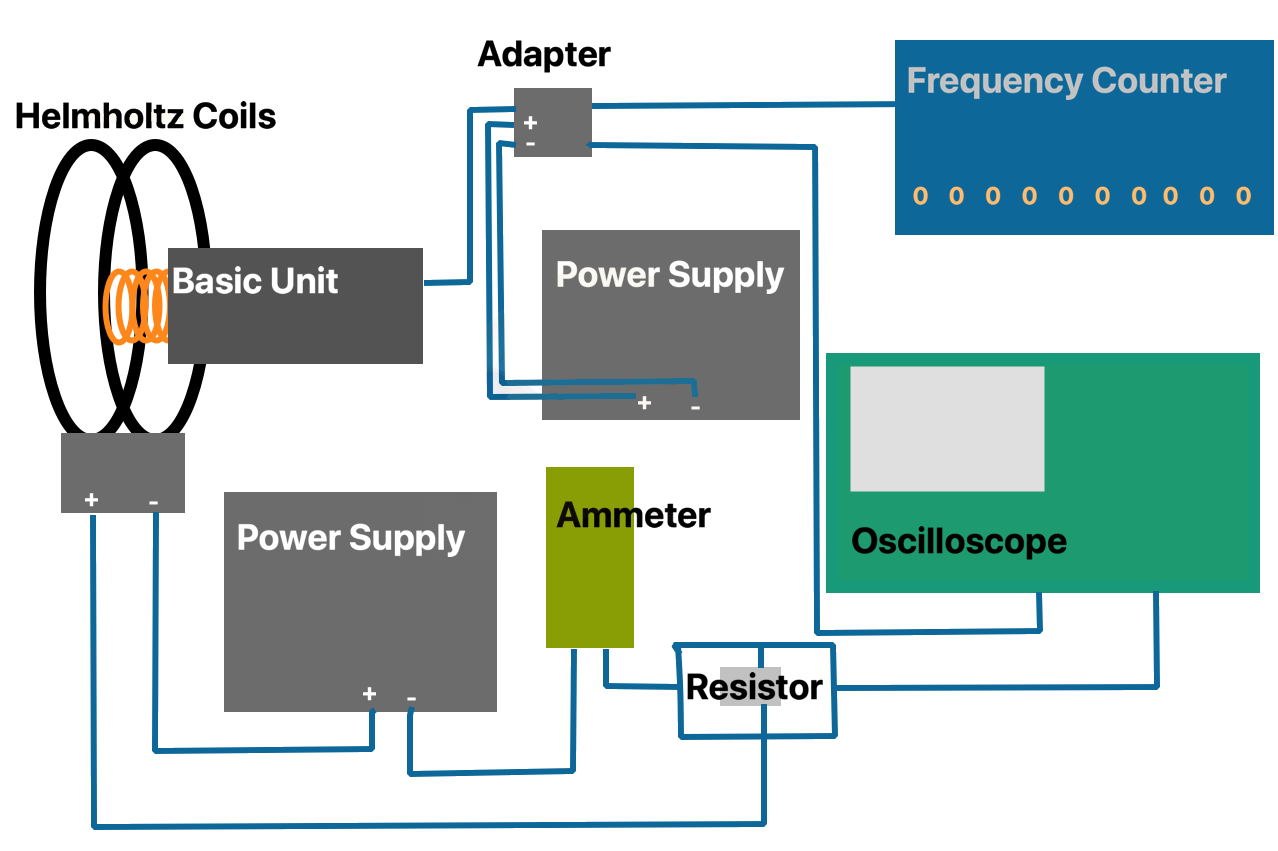
\includegraphics[width=1\textwidth]{Circuit_Diagram_P2Lab.png}
\captionof{figure}{Schematic of equipment used in experiment}
\label{Circuit_Diagram}
\end{figure}

\section{Data Analysis}
%Graphs, figures, and tables with captions
%Results with error analysis
%Calculate discrepancies from theory

\subsection{Frequency Dependence of Resonance Field}

\qq Voltage was compared to frequency to obtain a graphical
relationship for the frequency dependence of the resonance field. Such a relationship is shown below in figure \ref{FrequencyDependence}.
The amplitude of the voltage was obtained by measuring the peak-to-peak voltage from the oscilloscope and dividing it in half. The peak in the data distribution graphed in figure \ref{FrequencyDependence} is the resonance frequency for the
field. This value occurs at a voltage of 1.01 V and a frequency of
$4.18*10^7$ Hz. It is important to note that the electron spin
resonance device divides the frequency by a factor of a thousand, which is reflected in the measurements taken with the
 Hewlett-Packard frequency counter. Thus the measurements needed to be corrected before analysis is carried out, i.e. the
counter's frequency are multiplied by one thousand.

\begin{figure}[H]
\centering
% uncomment the line below to add image
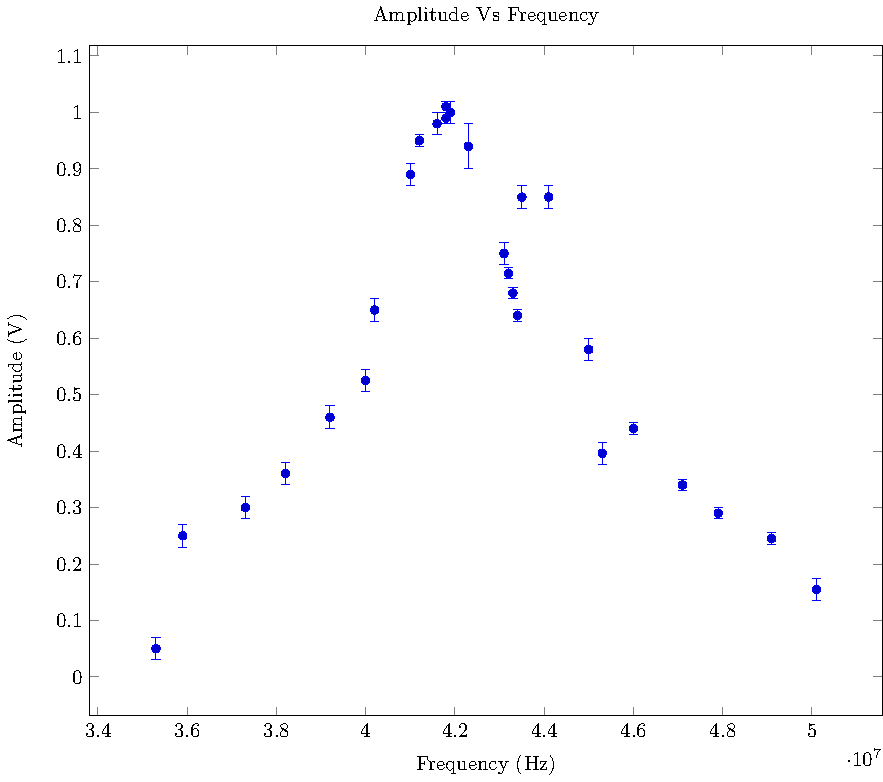
\includegraphics[width=1\textwidth]{Plots/ExpFreqVsVolt/freq_depen.pdf}
\captionof{figure}{Voltage amplitude versus frequency: a graphic representation of the frequency dependence
  of the resonance field.}
\label{FrequencyDependence}
\end{figure}

\subsection{Experimental Value of Gyromagnetic Ratio}
\qq The gyromagnetic ratio is calculated using equation \ref{eq:exp_gs},
where $\nu$ is the frequency, $h$ is Planck's constant, $\mu_B$ is the
Bohr magneton, and $B_0$ is the magnetic field strength.

\begin{equation}
\label{eq:exp_gs}
g_s = \frac{h \times \nu}{\mu_B \times B_0}
\end{equation}

\qq The magnetic field used in calculating equation \ref{eq:exp_gs}
must be calculated as well. It is determined from the measured current
using equation \ref{eq:exp_B}, where $\mu_0 = 4 \pi \times 10^{-7}
\frac{Vs}{Am}$, the number of turns is $n=320$, and the radius of the
coils is $r=6.8cm$.
\begin{equation}
\label{eq:exp_B}
B_0 = \mu_0 \left( \frac{4}{5} \right) ^{3/2} \times \frac{n}{r} \times I
\end{equation}

\qq Rather than measuring the current directly, the current is
calculated by measuring the voltage drop across a resistor, of which
the resistance is also measured. This calculation is shown below in
equation.
\begin{equation}
\label{eq:exp_I}
I = \frac{V}{R}
\end{equation}

\qq By substituting equation \ref{eq:exp_I} into equation \ref{eq:exp_B}, and
then substituting equation \ref{eq:exp_B} into equation
\ref{eq:exp_gs}, we arrive at an expression for the gyromagnetic ratio
in terms of known constants and measured quantities. This final
expression is shown in equation \ref{eq:exp_gs_combined}.
\begin{equation}
\label{eq:exp_gs_combined}
g_s = \frac{h \times \nu}{\mu_B \times \left( \mu_0 \left( \frac{4}{5}
  \right) ^{3/2} \times \frac{n}{r} \times \frac{V}{R} \right) }
\end{equation}

\subsection{Propagating Uncertainty in Gyromagnetic Ratio}
\qq The error in the experimental value of the gyromagnetic ratio is
determined by propagating uncertainty in equation
\ref{eq:exp_gs_combined}. There are no uncertainties associated with
fundamental constants such as $h$, $\mu_B$, and $\mu_0$. It is assumed
that the number of coil turns, $n$, also has no associated uncertainty
because it was reported in the manual as such. The uncertainty in the
radius is constant for all measurements, but the frequency, voltage,
and resistance will differ for each measurement. Equation
\ref{eq:delta_gs} shows this error propagation.

\begin{equation}
\label{eq:delta_gs}
\delta g_s = g_s \times
              \sqrt {
              		  \left( \frac{\delta \nu}{\nu} \right) ^2
              		+ \left( \frac{\delta r}{r} \right) ^2
              		+ \left( \frac{\delta V}{V} \right) ^2
              		+ \left( \frac{\delta R}{R} \right) ^2
					} \\ \\
\end{equation}

An example calculation for the value of $g_s$ and its propagated
uncertainty is shown below for a measurement taken with the large
coil:

\begin{align*}
g_s &= \frac
		{6.626 \times 10^{-34} \times  \left( 3 \times 10^7 \right) }
		{\mu_B \times \left( 4 \pi \times 10^{-7}
						     \left( \frac{4}{5} \right) ^{3/2}
						     \times \frac{320}{0.068}
						     \times \frac{0.44}{1.7} \right)
	     } \\
    &= 1.93
\end{align*}
%
Again, the associated uncertainty is as follows:
%
\begin{align*}
\delta g_s &=
		   g_s \times
              \sqrt {
              		  \left( \frac{1.00 \times 10^4 \text{Hz}}{3.00 \times 10^7 \text{Hz}} \right) ^2
              		+ \left( \frac{0.5 \text{cm}}{6.7 \text{cm}} \right) ^2
              		+ \left( \frac{0.1 \text{V}}{2 \text{V}} \right) ^2
              		+ \left( \frac{0.1 \Omega}{1.7 \Omega} \right) ^2
					} \\
		  &= 1.93 \times
              \sqrt {
              		  \left( 3.3 \times 10^{-4} \right) ^2
              		+ \left( 0.006 \right) ^2
              		+ \left( 0.05 \right) ^2
              		+ \left( 0.06 \right) ^2
					} \\
		  &= .15
\end{align*}

\newpage

We can calculate the discrepancy between the experimental and
theoretical values as follows. Recall the theoretical value of $g_s$
for DPPH is 2.0036, which is approximated as 2.00 due to the limited
precision of the experimental value.


\begin{align*}
\Delta g_s &= | g_{s_{exp}} - g_{s_{theo}} | \\ &= | 1.93 - 2.00 |
\\ &= 0.074 \\
\end{align*}

Evidently, this difference $\Delta g_s$ is less than $1 \sigma$, which is taken to be $\delta g_s = 0.15$.

\subsection{Rejection of Data}
\qq During the data-taking process for the "big coil", a measurement
at a particular frequency produced an experimental $g_s$ value that
seemed anomalous; most measurements fall between 1 and 4, but this
measurement is around 13. Chauvenet's criterion will be used to
determine if this datum should be discarded.

\qq If one assumes this measurement to be valid, the resultant average
and standard deviation are $2.59 \pm 2.91$ (quite an atrocity). The
measurement in question, 13.08, differs from the average by $4.49
\sigma$. If a Gaussian distribution is assumed for the $g_s$ values,
the probability of obtaining a measurement that differs from the mean
by this quantity is determined as follows:

\begin{align*}
Prob(\text{outside }  4.49 \sigma) &= 1 - Prob(\text{within } 4.49 \sigma) \\
							  &= 1 -  .9999994 \\
							  &= 0 \\
\end{align*}

\qq Since the probability of a measurement being withing $4.49 \sigma$
is so high, the probability of this measurement being outside this
interval is effectively zero. Therefore, we can discard the anomalous
datum with extremely high confidence.

\subsection{Determining Line Width of Resonance Signal}
\qq The quantity $\delta B_0$ is representative of an absorption line, and is
obtained when the energy is measured at a fixed frequency as function
of the magnetic field. The line width $\delta B_0$ is used as an
expression of the uncertainty in the energy of the transition. This is
best represented by the equation $\delta E = g \times \mu_0 \times
\delta B_0$. Using the uncertainty principle a relation is then found
for $\delta B_0$.

\begin{align*}
\delta B_0 = \frac{\hbar}{2 \times g_J \times \mu_B \times T},
\end{align*}
where T is the lifetime of the level and $g_J$ is the Land$\acute{e}$
factor.

\newpage

Experimentally $\delta B_0$ can be determined by equation \ref{eq:line_width}, where $\delta$I is represented as $\frac{\delta U}{U_{mod}} \times  I_{mod} \times 2\sqrt{2}$.

\begin{equation}
\label{eq:line_width}
\delta B_0 = B \times \left( \frac{\delta I}{I_{mod}} \right)
\end{equation}
%
This first requires an intermittent calculation of $\delta I$ as follows:
%
\begin{align*}
\delta I &= \frac{\delta U}{U_{mod}} \times  I_{mod} \times 2\sqrt{2} \\
         &= \frac{0.55}{2} \times 0.156 \times 2\sqrt{2} \\
         &= 0.121
\end{align*}
%
Substituting into equation \ref{eq:line_width} yields the following calculation:
%
\begin{align*}
\delta B_0 &= B \times \left( \frac {\delta I} {I_{mod}} \right) \\
           &= 6.23 \times 10^{-4} \times \left( \frac {0.121} {0.156} \right) \\
           &= 4.85 \times 10^{-4} T \\
           &= 0.49 mT
\end{align*}


\section{Results: Discrepancies and Uncertainties}
%Discuss results and uncertainties
%Compare results with theory
%Approximations to theory

\subsection{Discrepancy in Gyromagnetic Ratio}
\qq The discrepancy between the experimental and theoretical values of G for
each of the coils can be calculated with \( \Delta g_s = | g_{s_t} - g_{s_e} |
\), where \( g_{s_t} \) is the theoretical value of \( g_s \) and \( g_{s_e} \)
is the experimental value. The discrepancy in the value of \( g_s \) for the
small coil is:

\begin{align*}
  \Delta g_{s_{\text{small}}} =& \left| (2.00) - (1.44) \right| \\
   =& 0.56 \\
\end{align*}

Since the standard deviation of the calculated values is
\( \sigma_{g_s, \text{small}} = 0.393 \), the experimental value of \( g_s \) is $$
\frac{\Delta g_{s_{\text{small}}}}{\sigma_{g_s, \text{small}}} = \frac{0.56}{0.393} = 1.42
\sigma $$ from the theoretical value of $g_s = 2.00$.

\newpage

\qq The discrepancies for the medium and big coils were calculated in the same
manner, and the results are detailed in table \ref{tab:discrepancyG}. The results
from the three coils are then used to calculate a true average value of \( g_s
\). The uncertainty in this value is the standard deviation of the mean, computed from all the data
points across all the coils.

\begin{table}[H]
  \caption{The discrepancies between the theoretical and experimental values for
    \( g_s \) for the small, medium, and big coils as well as the average value
    of \( g_s \).}
  \begin{center}
    \begin{tabular}{|l|l|l|l|l|l|}
      \hline
      Coil & Theoretical \( g_s \) & Experimental \( g_s \) & \( \Delta g_s \) &
                                                                                 Standard
                                                                                 Deviation
                                                                                 (\(
                                                                                 \sigma
                                                                                 \)) &
                                                                                 \(
                                                                                 \sigma
                                                                                 \Delta
                                                                                 g_s
                                                                                 \)
      \\
      \hline
      Small & 2.00 & 1.44 & 0.56 & 0.39 & 1.4 \( \sigma \) \\
      Medium & 2.00 & 1.16 & 0.84 & 0.13 & 6.7 \( \sigma \) \\
      Big & 2.00 & 1.89 & 0.11 & 0.83 & 0.13 \( \sigma \) \\
      \hline
      Average & 2.00 & 1.37 & 0.63 & 0.47 & 1.3 \( \sigma \) \\
      \hline
    \end{tabular}
  \end{center}
  \label{tab:discrepancyG}
\end{table}


\subsection{Discrepancy in Line Width}
\qq The line width itself is representative of an error in the energy,
as discussed above. Therefore, an uncertainty will not be calculated
in the line width, as it is already a calculation involving
uncertainties of constituent quantities. However, the experimental
value can be compared to an acceptable range given by literature
sources. The experimental line width was determined to be $\delta B_0
= 0.49 mT$. The range given for theoretical line width was [0.15,0.81]
mT, thus the experimental value is within the acceptable range.

\section{Sources of Error}
%Discuss the radius/seperation
%Discuss the equipment heating
\qq An ideal Helmholtz coil has a separation distance equal to its coil radii. The width of the "basic unit" module, which holds
the coil samples, was larger than the radius of the coil. Thus the
separation distance was limited to this width, and was larger than the coil radius. This restriction of the experimental set-up results in a magnetic field systematically lower than that indicated by calculations, as a true Helmholtz coil is
designed with such a separation distance in order to maximize constructive interference of the constituent coils' fields. Any deviation from this set-up will result in a weaker field.  Furthermore,
because the magnetic field is systematically lower than the
prediction, the calculated $g_s$ is systematically higher that calculations predits, since the two quantities are inversely proportional.

\qq Both the Helmholtz coil and the 1 $M \Omega$ resistor began heating up throughout the course of the experiment. The heating of the equipment
causes energy loss in the system as the
thermal energy transfers from the system to the surrounding region. This means that less energy is translated into the magnetic field, and since this quantity is directly proportional to the calculation of $g_s$, the value for $g_s$ will be systematically lower than predicted. As the
resistor heats up, its resistivity and thus resistance increases, however this effect was mitigated in the calculations by repeatedly measuring the resistance of the resistor, before every trial, and using each resistance for its respective calculation of $g_s$.

\section{Conclusion}
%Brief summary, discussion of results and theory
\qq Within the experiment, the value of \( g_s \) was calculated for small,
medium, and big coils, and these values were used to determine an average
\( g_s \) value. The \( g_s \) value for the small coil was calculated to be
\( 1.44 \pm \num{6.5e-2} \) with a discrepancy from the theoretical value of
\( 1.4 \sigma \). The \( g_s \) value of the medium coil is
\( 1.16 \pm \num{1.8e-2} \) with a discrepancy of \( 6.7 \sigma \), and the
\( g_s \) value of the big coil is \( 1.89 \pm \num{2.1e-1} \) with a
discrepancy of \( 0.13 \sigma \). The average \( g_s \) value is
\( 1.37 \pm 0.05 \) with a discrepancy of \( 1.3 \sigma \). Additionally, the
resonant frequency of DPPH was determined graphically from Figure
\ref{FrequencyDependence} to be \SI{4.1e7}{\hertz}.

\section{Appendices}

\subsection{Appendix A: Data}

\subsubsection{Frequency \& Voltage}

\begin{table}[H]
  \caption{The recorded frequencies and corresponding voltages used to determine
    resonant frequency. These values are plotted in Figure
    \ref{FrequencyDependence}.}
  \begin{center}
    \begin{tabular}{|l|l|}
      \hline
      Frequency (\si{\mega\hertz}) & Voltage (\si{\volt}) \\
      \hline
      35 \( \pm \) 0.01 & 0.05  \( \pm \) 0.02 \\
      40 \( \pm \) 0.01 & 0.53  \( \pm \) 0.02 \\
      45 \( \pm \) 0.01 & 0.40  \( \pm \) 0.02 \\
      50 \( \pm \) 0.01 & 0.16  \( \pm \) 0.02 \\
      35 \( \pm \) 0.01 & 0.25  \( \pm \) 0.02 \\
      37 \( \pm \) 0.01 & 0.30  \( \pm \) 0.02 \\
      38 \( \pm \) 0.01 & 0.36  \( \pm \) 0.02 \\
      39 \( \pm \) 0.01 & 0.46  \( \pm \) 0.02 \\
      40 \( \pm \) 0.01 & 0.65  \( \pm \) 0.02 \\
      41 \( \pm \) 0.01 & 0.89  \( \pm \) 0.02 \\
      41 \( \pm \) 0.01 & 0.98  \( \pm \) 0.02 \\
      43 \( \pm \) 0.01 & 0.75  \( \pm \) 0.02 \\
      44 \( \pm \) 0.01 & 0.85  \( \pm \) 0.02 \\
      45 \( \pm \) 0.01 & 0.58  \( \pm \) 0.02 \\
      46 \( \pm \) 0.01 & 0.44  \( \pm \) 0.01 \\
      47 \( \pm \) 0.01 & 0.34  \( \pm \) 0.01 \\
      47 \( \pm \) 0.01 & 0.29  \( \pm \) 0.01 \\
      49 \( \pm \) 0.01 & 0.25  \( \pm \) 0.01 \\
      41 \( \pm \) 0.01 & 0.95  \( \pm \) 0.01 \\
      41 \( \pm \) 0.01 & 0.99  \( \pm \) 0.01 \\
      43 \( \pm \) 0.01 & 0.72  \( \pm \) 0.01 \\
      41 \( \pm \) 0.20 & 1.01  \( \pm \) 0.01 \\
      41 \( \pm \) 0.10 & 1.00  \( \pm \) 0.02 \\
      42 \( \pm \) 0.01 & 0.94  \( \pm \) 0.04 \\
      43 \( \pm \) 0.01 & 0.64  \( \pm \) 0.01 \\
      43 \( \pm \) 0.01 & 0.68  \( \pm \) 0.01 \\
      43 \( \pm \) 0.01 & 0.85  \( \pm \) 0.02 \\
      \hline
    \end{tabular}
  \end{center}
  \label{tab:freqVolt}
\end{table}

\subsubsection{Small Coil}

\begin{table}[H]
  \caption{The data collected from measurements with the small coil and data
    calculated from those measurements.}
  \begin{center}
    \begin{tabular}{|l|l|l|l|}
      \hline
      Frequency (\si{\mega\hertz}) & Voltage (\si{\volt}) & Resistance
                                                            (\si{\ohm}) &
                                                                          G-Factor
      \\
      \hline
      75 \( \pm \) 0.01 & 1.4 \( \pm \) 0.2 & 1.6 \( \pm \) 0.1 & 1.43 \( \pm \) \num{2.22e-01} \\
      75 \( \pm \) 0.01 & 1.5 \( \pm \) 0.2 & 1.6 \( \pm \) 0.1 & 1.33 \( \pm \) \num{1.96e-01} \\
      75 \( \pm \) 0.01 & 2.6 \( \pm \) 0.2 & 1.6 \( \pm \) 0.1 & 0.77 \( \pm \) \num{7.61e-02} \\
      75 \( \pm \) 0.01 & 2.9 \( \pm \) 0.2 & 1.6 \( \pm \) 0.1 & 0.69 \( \pm \) \num{6.41e-02} \\
      80 \( \pm \) 0.01 & 1.5 \( \pm \) 0.1 & 1.5 \( \pm \) 0.1 & 1.33 \( \pm \) \num{1.25e-01} \\
      80 \( \pm \) 0.01 & 1.5 \( \pm \) 0.1 & 1.5 \( \pm \) 0.1 & 1.33 \( \pm \) \num{1.25e-01} \\
      80 \( \pm \) 0.01 & 1.5 \( \pm \) 0.1 & 1.5 \( \pm \) 0.1 & 1.33 \( \pm \) \num{1.25e-01} \\
      80 \( \pm \) 0.01 & 2.8 \( \pm \) 0.1 & 1.5 \( \pm \) 0.1 & 0.71 \( \pm \) \num{5.39e-02} \\
      85 \( \pm \) 0.01 & 1.2 \( \pm \) 0.1 & 1.5 \( \pm \) 0.1 & 1.84 \( \pm \) \num{2.02e-01} \\
      85 \( \pm \) 0.01 & 1.1 \( \pm \) 0.1 & 1.5 \( \pm \) 0.1 & 2.02 \( \pm \) \num{2.35e-01} \\
      85 \( \pm \) 0.01 & 2.0 \( \pm \) 0.1 & 1.5 \( \pm \) 0.1 & 1.06 \( \pm \) \num{8.83e-02} \\
      85 \( \pm \) 0.01 & 2.0 \( \pm \) 0.1 & 1.5 \( \pm \) 0.1 & 1.06 \( \pm \) \num{8.83e-02} \\
      90 \( \pm \) 0.01 & 2.2 \( \pm \) 0.1 & 1.5 \( \pm \) 0.1 & 1.05 \( \pm \) \num{8.52e-02} \\
      90 \( \pm \) 0.01 & 2.0 \( \pm \) 0.1 & 1.5 \( \pm \) 0.1 & 1.13 \( \pm \) \num{9.39e-02} \\
      90 \( \pm \) 0.01 & 1.3 \( \pm \) 0.1 & 1.5 \( \pm \) 0.1 & 1.80 \( \pm \) \num{1.88e-01} \\
      90 \( \pm \) 0.01 & 1.2 \( \pm \) 0.1 & 1.5 \( \pm \) 0.1 & 1.88 \( \pm \) \num{2.00e-01} \\
      95 \( \pm \) 0.01 & 1.4 \( \pm \) 0.1 & 1.6 \( \pm \) 0.1 & 1.80 \( \pm \) \num{1.71e-01} \\
      95 \( \pm \) 0.01 & 1.4 \( \pm \) 0.1 & 1.6 \( \pm \) 0.1 & 1.80 \( \pm \) \num{1.71e-01} \\
      95 \( \pm \) 0.01 & 2.1 \( \pm \) 0.1 & 1.6 \( \pm \) 0.1 & 1.20 \( \pm \) \num{9.45e-02} \\
      95 \( \pm \) 0.01 & 2.1 \( \pm \) 0.1 & 1.6 \( \pm \) 0.1 & 1.20 \( \pm \) \num{9.45e-02} \\
      10 \( \pm \) 0.01 & 2.2 \( \pm \) 0.1 & 1.6 \( \pm \) 0.1 & 1.21 \( \pm \) \num{9.35e-02} \\
      10 \( \pm \) 0.01 & 2.2 \( \pm \) 0.1 & 1.6 \( \pm \) 0.1 & 1.24 \( \pm \) \num{9.64e-02} \\
      10 \( \pm \) 0.01 & 1.5 \( \pm \) 0.1 & 1.6 \( \pm \) 0.1 & 1.78 \( \pm \) \num{1.62e-01} \\
      10 \( \pm \) 0.01 & 1.5 \( \pm \) 0.1 & 1.6 \( \pm \) 0.1 & 1.84 \( \pm \) \num{1.71e-01} \\
      10 \( \pm \) 0.01 & 1.5 \( \pm \) 0.1 & 1.6 \( \pm \) 0.1 & 1.86 \( \pm \) \num{1.70e-01} \\
      10 \( \pm \) 0.01 & 1.5 \( \pm \) 0.1 & 1.6 \( \pm \) 0.1 & 1.86 \( \pm \) \num{1.70e-01} \\
      10 \( \pm \) 0.01 & 2.3 \( \pm \) 0.1 & 1.6 \( \pm \) 0.1 & 1.21 \( \pm \) \num{9.25e-02} \\
      10 \( \pm \) 0.01 & 2.3 \( \pm \) 0.1 & 1.6 \( \pm \) 0.1 & 1.21 \( \pm \) \num{9.25e-02} \\
      11 \( \pm \) 0.01 & 2.4 \( \pm \) 0.1 & 1.5 \( \pm \) 0.1 & 1.17 \( \pm \) \num{9.24e-02} \\
      11 \( \pm \) 0.01 & 1.6 \( \pm \) 0.1 & 1.5 \( \pm \) 0.1 & 1.72 \( \pm \) \num{1.57e-01} \\
      12 \( \pm \) 0.01 & 1.7 \( \pm \) 0.1 & 1.6 \( \pm \) 0.1 & 1.86 \( \pm \) \num{1.61e-01} \\
      12 \( \pm \) 0.01 & 2.4 \( \pm \) 0.1 & 1.6 \( \pm \) 0.1 & 1.28 \( \pm \) \num{9.58e-02} \\
      12 \( \pm \) 0.01 & 2.4 \( \pm \) 0.1 & 1.6 \( \pm \) 0.1 & 1.36 \( \pm \) \num{1.03e-01} \\
      12 \( \pm \) 0.01 & 1.5 \( \pm \) 0.1 & 1.6 \( \pm \) 0.1 & 2.13 \( \pm \) \num{1.95e-01} \\
      13 \( \pm \) 0.01 & 1.6 \( \pm \) 0.1 & 1.6 \( \pm \) 0.1 & 2.08 \( \pm \) \num{1.84e-01} \\
      13 \( \pm \) 0.01 & 2.4 \( \pm \) 0.1 & 1.6 \( \pm \) 0.1 & 1.39 \( \pm \) \num{1.04e-01} \\
      \hline
    \end{tabular}
  \end{center}
  \label{tab:smallCoil}
\end{table}

\subsubsection{Medium Coil}

\begin{table}[H]
  \caption{The data collected from measurements with the medium coil and data
    calculated from those measurements.}
  \begin{center}
    \begin{tabular}{|l|l|l|l|}
      \hline
      Frequency (\si{\mega\hertz}) & Voltage (\si{\volt}) & Resistance (\si{\ohm}) & G-Factor \\
      \hline
      43 \( \pm \) 0.01 & 0.90 \( \pm \) 0.10 & 1.5 \( \pm \) 0.1 & 1.18 \( \pm \) \num{1.53e-01} \\
      44 \( \pm \) 0.01 & 0.80 \( \pm \) 0.10 & 1.2 \( \pm \) 0.1 & 1.11 \( \pm \) \num{1.66e-01} \\
      44 \( \pm \) 0.01 & 0.82 \( \pm \) 0.10 & 1.2 \( \pm \) 0.1 & 1.08 \( \pm \) \num{1.60e-01} \\
      44 \( \pm \) 0.01 & 0.82 \( \pm \) 0.10 & 1.2 \( \pm \) 0.1 & 1.08 \( \pm \) \num{1.60e-01} \\
      44 \( \pm \) 0.01 & 0.80 \( \pm \) 0.10 & 1.2 \( \pm \) 0.1 & 1.11 \( \pm \) \num{1.66e-01} \\
      45 \( \pm \) 0.01 & 0.96 \( \pm \) 0.04 & 1.2 \( \pm \) 0.1 & 0.94 \( \pm \) \num{8.72e-02} \\
      45 \( \pm \) 0.01 & 0.92 \( \pm \) 0.04 & 1.2 \( \pm \) 0.1 & 0.98 \( \pm \) \num{9.18e-02} \\
      45 \( \pm \) 0.01 & 0.80 \( \pm \) 0.04 & 1.2 \( \pm \) 0.1 & 1.12 \( \pm \) \num{1.09e-01} \\
      45 \( \pm \) 0.01 & 0.76 \( \pm \) 0.04 & 1.2 \( \pm \) 0.1 & 1.18 \( \pm \) \num{1.17e-01} \\
      46 \( \pm \) 0.01 & 0.96 \( \pm \) 0.04 & 1.4 \( \pm \) 0.1 & 1.11 \( \pm \) \num{9.21e-02} \\
      46 \( \pm \) 0.01 & 0.94 \( \pm \) 0.04 & 1.4 \( \pm \) 0.1 & 1.14 \( \pm \) \num{9.46e-02} \\
      46 \( \pm \) 0.01 & 0.80 \( \pm \) 0.04 & 1.4 \( \pm \) 0.1 & 1.34 \( \pm \) \num{1.17e-01} \\
      46 \( \pm \) 0.01 & 0.84 \( \pm \) 0.04 & 1.4 \( \pm \) 0.1 & 1.27 \( \pm \) \num{1.09e-01} \\
      47 \( \pm \) 0.01 & 0.96 \( \pm \) 0.04 & 1.3 \( \pm \) 0.1 & 1.06 \( \pm \) \num{9.28e-02} \\
      47 \( \pm \) 0.01 & 1.00 \( \pm \) 0.04 & 1.3 \( \pm \) 0.1 & 1.02 \( \pm \) \num{8.83e-02} \\
      47 \( \pm \) 0.01 & 0.82 \( \pm \) 0.04 & 1.3 \( \pm \) 0.1 & 1.24 \( \pm \) \num{1.13e-01} \\
      47 \( \pm \) 0.01 & 0.84 \( \pm \) 0.04 & 1.3 \( \pm \) 0.1 & 1.21 \( \pm \) \num{1.10e-01} \\
      48 \( \pm \) 0.01 & 0.84 \( \pm \) 0.04 & 1.3 \( \pm \) 0.1 & 1.24 \( \pm \) \num{1.12e-01} \\
      48 \( \pm \) 0.01 & 0.82 \( \pm \) 0.04 & 1.3 \( \pm \) 0.1 & 1.27 \( \pm \) \num{1.15e-01} \\
      48 \( \pm \) 0.01 & 1.00 \( \pm \) 0.04 & 1.3 \( \pm \) 0.1 & 1.04 \( \pm \) \num{9.00e-02} \\
      48 \( \pm \) 0.01 & 1.00 \( \pm \) 0.04 & 1.3 \( \pm \) 0.1 & 1.04 \( \pm \) \num{9.00e-02} \\
      49 \( \pm \) 0.01 & 1.00 \( \pm \) 0.04 & 1.3 \( \pm \) 0.1 & 1.06 \( \pm \) \num{9.19e-02} \\
      49 \( \pm \) 0.01 & 1.00 \( \pm \) 0.04 & 1.3 \( \pm \) 0.1 & 1.06 \( \pm \) \num{9.19e-02} \\
      49 \( \pm \) 0.01 & 0.90 \( \pm \) 0.04 & 1.3 \( \pm \) 0.1 & 1.18 \( \pm \) \num{1.05e-01} \\
      49 \( \pm \) 0.01 & 0.86 \( \pm \) 0.04 & 1.3 \( \pm \) 0.1 & 1.23 \( \pm \) \num{1.11e-01} \\
      50 \( \pm \) 0.01 & 0.90 \( \pm \) 0.04 & 1.2 \( \pm \) 0.1 & 1.11 \( \pm \) \num{1.05e-01} \\
      50 \( \pm \) 0.01 & 0.88 \( \pm \) 0.04 & 1.2 \( \pm \) 0.1 & 1.14 \( \pm \) \num{1.08e-01} \\
      50 \( \pm \) 0.01 & 1.00 \( \pm \) 0.04 & 1.2 \( \pm \) 0.1 & 1.00 \( \pm \) \num{9.26e-02} \\
      50 \( \pm \) 0.01 & 1.00 \( \pm \) 0.04 & 1.2 \( \pm \) 0.1 & 1.00 \( \pm \) \num{9.26e-02} \\
      51 \( \pm \) 0.01 & 0.95 \( \pm \) 0.10 & 1.3 \( \pm \) 0.1 & 1.16 \( \pm \) \num{1.51e-01} \\
      51 \( \pm \) 0.01 & 1.00 \( \pm \) 0.10 & 1.3 \( \pm \) 0.1 & 1.10 \( \pm \) \num{1.39e-01} \\
      \hline
    \end{tabular}
  \end{center}
  \label{tab:medCoil}
\end{table}

\begin{table}[H]
  \begin{center}
    \begin{tabular}{|l|l|l|l|}
      \hline
      Frequency (\si{\mega\hertz}) & Voltage (\si{\volt}) & Resistance (\si{\ohm}) & G-Factor \\
      \hline
      55 \( \pm \) 0.01 & 1.00 \( \pm \) 0.10 & 1.4 \( \pm \) 0.1 & 1.28 \( \pm \) \num{1.58e-01} \\
      55 \( \pm \) 0.01 & 0.96 \( \pm \) 0.10 & 1.4 \( \pm \) 0.1 & 1.34 \( \pm \) \num{1.69e-01} \\
      60 \( \pm \) 0.01 & 0.96 \( \pm \) 0.04 & 1.3 \( \pm \) 0.1 & 1.35 \( \pm \) \num{1.18e-01} \\
      60 \( \pm \) 0.01 & 0.94 \( \pm \) 0.04 & 1.3 \( \pm \) 0.1 & 1.38 \( \pm \) \num{1.21e-01} \\
      65 \( \pm \) 0.01 & 0.90 \( \pm \) 0.04 & 1.3 \( \pm \) 0.1 & 1.56 \( \pm \) \num{1.39e-01} \\
      40 \( \pm \) 0.01 & 0.74 \( \pm \) 0.04 & 1.3 \( \pm \) 0.1 & 1.17 \( \pm \) \num{1.10e-01} \\
      40 \( \pm \) 0.01 & 0.68 \( \pm \) 0.04 & 1.3 \( \pm \) 0.1 & 1.27 \( \pm \) \num{1.23e-01} \\
      40 \( \pm \) 0.01 & 0.84 \( \pm \) 0.04 & 1.3 \( \pm \) 0.1 & 1.03 \( \pm \) \num{9.29e-02} \\
      40 \( \pm \) 0.01 & 0.82 \( \pm \) 0.04 & 1.3 \( \pm \) 0.1 & 1.05 \( \pm \) \num{9.59e-02} \\
      35 \( \pm \) 0.01 & 0.60 \( \pm \) 0.04 & 1.3 \( \pm \) 0.1 & 1.26 \( \pm \) \num{1.28e-01} \\
      35 \( \pm \) 0.01 & 0.60 \( \pm \) 0.04 & 1.3 \( \pm \) 0.1 & 1.26 \( \pm \) \num{1.28e-01} \\
      35 \( \pm \) 0.01 & 0.76 \( \pm \) 0.04 & 1.3 \( \pm \) 0.1 & 1.00 \( \pm \) \num{9.28e-02} \\
      35 \( \pm \) 0.01 & 0.68 \( \pm \) 0.04 & 1.3 \( \pm \) 0.1 & 1.11 \( \pm \) \num{1.08e-01} \\
      30 \( \pm \) 0.01 & 0.60 \( \pm \) 0.04 & 1.4 \( \pm \) 0.1 & 1.16 \( \pm \) \num{1.13e-01} \\
      30 \( \pm \) 0.01 & 0.52 \( \pm \) 0.04 & 1.4 \( \pm \) 0.1 & 1.34 \( \pm \) \num{1.41e-01} \\
      30 \( \pm \) 0.01 & 0.60 \( \pm \) 0.04 & 1.4 \( \pm \) 0.1 & 1.16 \( \pm \) \num{1.13e-01} \\
      30 \( \pm \) 0.01 & 0.60 \( \pm \) 0.04 & 1.4 \( \pm \) 0.1 & 1.16 \( \pm \) \num{1.13e-01} \\
      \hline
    \end{tabular}
  \end{center}
\end{table}

\subsubsection{Big Coil}

\begin{table}[H]
  \caption{The data collected from measurements with the big coil and data
    calculated from those measurements. The omitted data point is highlighted.}
  \begin{center}
    \begin{tabular}{|l|l|l|l|}
      \hline
      Frequency (\si{\mega\hertz}) & Voltage (\si{\volt}) & Resistance (\si{\ohm}) & G-Factor \\
      \hline
      30 \( \pm \) 0.01 & 0.44 \( \pm \) 0.08 & 1.7 \( \pm \) 0.1 & 1.93 \( \pm \) \num{3.69e-01} \\
      30 \( \pm \) 0.01 & 0.60 \( \pm \) 0.08 & 1.7 \( \pm \) 0.1 & 1.41 \( \pm \) \num{2.06e-01} \\
      30 \( \pm \) 0.01 & 0.56 \( \pm \) 0.08 & 1.7 \( \pm \) 0.1 & 1.52 \( \pm \) \num{2.34e-01} \\
      30 \( \pm \) 0.01 & 0.50 \( \pm \) 0.08 & 1.7 \( \pm \) 0.1 & 1.70 \( \pm \) \num{2.89e-01} \\
      25 \( \pm \) 0.01 & 0.40 \( \pm \) 0.10 & 1.8 \( \pm \) 0.1 & 1.87 \( \pm \) \num{4.79e-01} \\
      25 \( \pm \) 0.01 & 0.44 \( \pm \) 0.10 & 1.8 \( \pm \) 0.1 & 1.70 \( \pm \) \num{3.98e-01} \\
      25 \( \pm \) 0.01 & 0.40 \( \pm \) 0.10 & 1.8 \( \pm \) 0.1 & 1.87 \( \pm \) \num{4.79e-01} \\
      25 \( \pm \) 0.01 & 0.50 \( \pm \) 0.10 & 1.8 \( \pm \) 0.1 & 1.50 \( \pm \) \num{3.11e-01} \\
      20 \( \pm \) 0.01 & 0.20 \( \pm \) 0.04 & 1.9 \( \pm \) 0.1 & 3.17 \( \pm \) \num{6.54e-01} \\
      20 \( \pm \) 0.01 & 0.40 \( \pm \) 0.04 & 1.9 \( \pm \) 0.1 & 1.58 \( \pm \) \num{1.79e-01} \\
      20 \( \pm \) 0.01 & 0.36 \( \pm \) 0.04 & 1.9 \( \pm \) 0.1 & 1.76 \( \pm \) \num{2.16e-01} \\
      20 \( \pm \) 0.01 & 0.40 \( \pm \) 0.04 & 1.9 \( \pm \) 0.1 & 1.58 \( \pm \) \num{1.79e-01} \\
      \hline
15 \( \pm \) 0.01 & 0.04 \( \pm \) 0.01 & 2.1 \( \pm \) 0.1 & 13.1 \( \pm \) \num{3.33e+00} \\
      \hline
      15 \( \pm \) 0.01 & 0.48 \( \pm \) 0.08 & 2.1 \( \pm \) 0.1 & 1.09 \( \pm \) \num{1.89e-01} \\
      15 \( \pm \) 0.01 & 0.40 \( \pm \) 0.04 & 2.1 \( \pm \) 0.1 & 1.31 \( \pm \) \num{1.45e-01} \\
      15 \( \pm \) 0.01 & 0.12 \( \pm \) 0.04 & 2.1 \( \pm \) 0.1 & 4.36 \( \pm \) \num{1.47e+00} \\
      \hline
    \end{tabular}
  \end{center}
  \label{tab:bigCoil}
\end{table}

\subsection{Appendix B: Source Code}

\subsubsection{Error Propagation and Data Processing}

\inputminted{julia}{Code/calcData.jl}

\end{document}
